\documentclass{beamer}
\usepackage[utf8]{inputenc}
\usepackage{multimedia}
\usepackage{template}
\usepackage{colortbl}
\usepackage{epstopdf}
\mode<article> % only for the article version
{
  \usepackage{fullpage}
  \usepackage{hyperref}
}
\graphicspath{{img/}}

\title[Uma implementação \textit{MapReduce} sobre Akka - Caso LRIT.]{Uma implementação \textit{MapReduce} sobre Akka - Caso LRIT.}
\author[Jonas Ferreira]{Jonas Ferreira da Silva Medeiros De La Cerda}
\date[Dezembro/2015]{\today}
\institute[UFF]{Universidade Federal Fluminense}

\begin{document} 
 
\titlepage

\section{Introdução}
	\subsection{LRIT - Long Range Identification and Tracking}
		\begin{frame}{LRIT - O que é?}
			\begin{itemize}
				\item Sistema estabelecido pela IMO (\textit{International Maritime Organization}) visando à \textbf{segurança} (\textit{security}) e \textbf{salvaguarda} (\textit{safety}) da vida humana ao mar;
				\item Obrigatório aos países signatários da convenção SOLAS (em torno de 200 nações) para as \textbf{embarcações mercantes} acima de uma determinada tonelagem.
			\end{itemize}
		\end{frame}

		\begin{frame}{LRIT - O que faz?}
		Permite o intercâmbio de informações de posições dos \textbf{navios mercantes} entre os governos contratantes.
			\begin{itemize}
				\item Monitorar áreas;
				\item Monitorar embarcações;
				\item Incidentes SAR (\textit{Search and Rescue});
				\item Interrogar embarcações.
			\end{itemize}
		\end{frame}

		\begin{frame}{LRIT - Overview}
			\begin{figure}[H]
				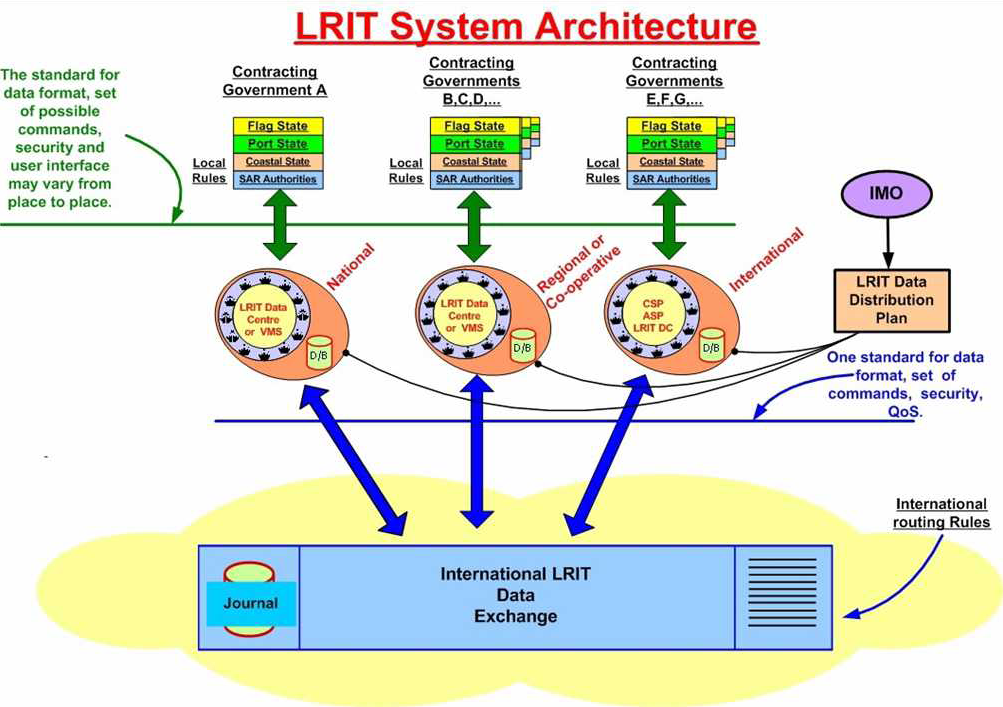
\includegraphics[scale=0.33]{img/lrit.png}
				\caption{Visão geral do sistema LRIT.}
				\label{fig:overview}
			\end{figure}
		\end{frame}

		\begin{frame}{LRIT - Características}
			\begin{itemize}
			\item Troca de mensagens assíncrona;
			\item Funciona sobre internet utilizando SOAP/XML e HTTPS;
			\item Requisitos de desempenho e disponibilidade;
			\item Tecnologicamente agnóstico.
			\end{itemize}
		\end{frame}

		\begin{frame}{LRIT - Brasil}
			\begin{itemize}
			\item JavaEE;
			\item JBoss;
			\item EJBs, MDBs, apache httpd (mod\_jk);
			\item PostgreSQL e PostGIS.
			\end{itemize}
		\end{frame}

		\begin{frame}{LRIT - Reúso}
			\begin{itemize}
				\item A mesma arquitetura e componentes podem ser reinstanciados para outros tipos de veículos.
				\item Volume de dados a ser processado (tanto em tempo real quanto em lote) pode crescer.
				\item Adequações ao processamento devem ser feitas a fim de suportar demandas maiores.
			\end{itemize}
		\end{frame}

	\subsection{MapReduce}
		\begin{frame}{MapReduce\cite{google_mapreduce}}
		\begin{itemize}
			\item Modelo de programação e implementação para processar grandes conjuntos de dados;
			\item Baseado em construtos da programação funcional: \textit{Map} e \textit{Reduce}.
			\item Recebe um conjunto de chaves e valores, produz um conjunto de chaves e valores.
		\end{itemize}
		\end{frame}

		\begin{frame}{MapReduce - Overview}
			\begin{figure}[H]
				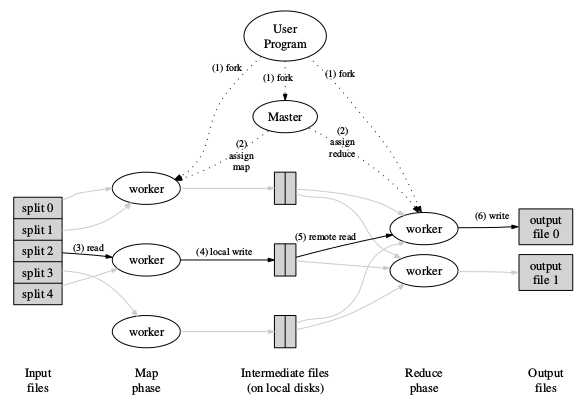
\includegraphics[scale=0.5]{img/mapreduce_original_overview.png}
				\caption{MapReduce overview\cite{google_mapreduce}}
				\label{fig:mapreduce_example}
			\end{figure}
		\end{frame}

		\begin{frame}{MapReduce - Exemplo}
			\begin{figure}[H]
				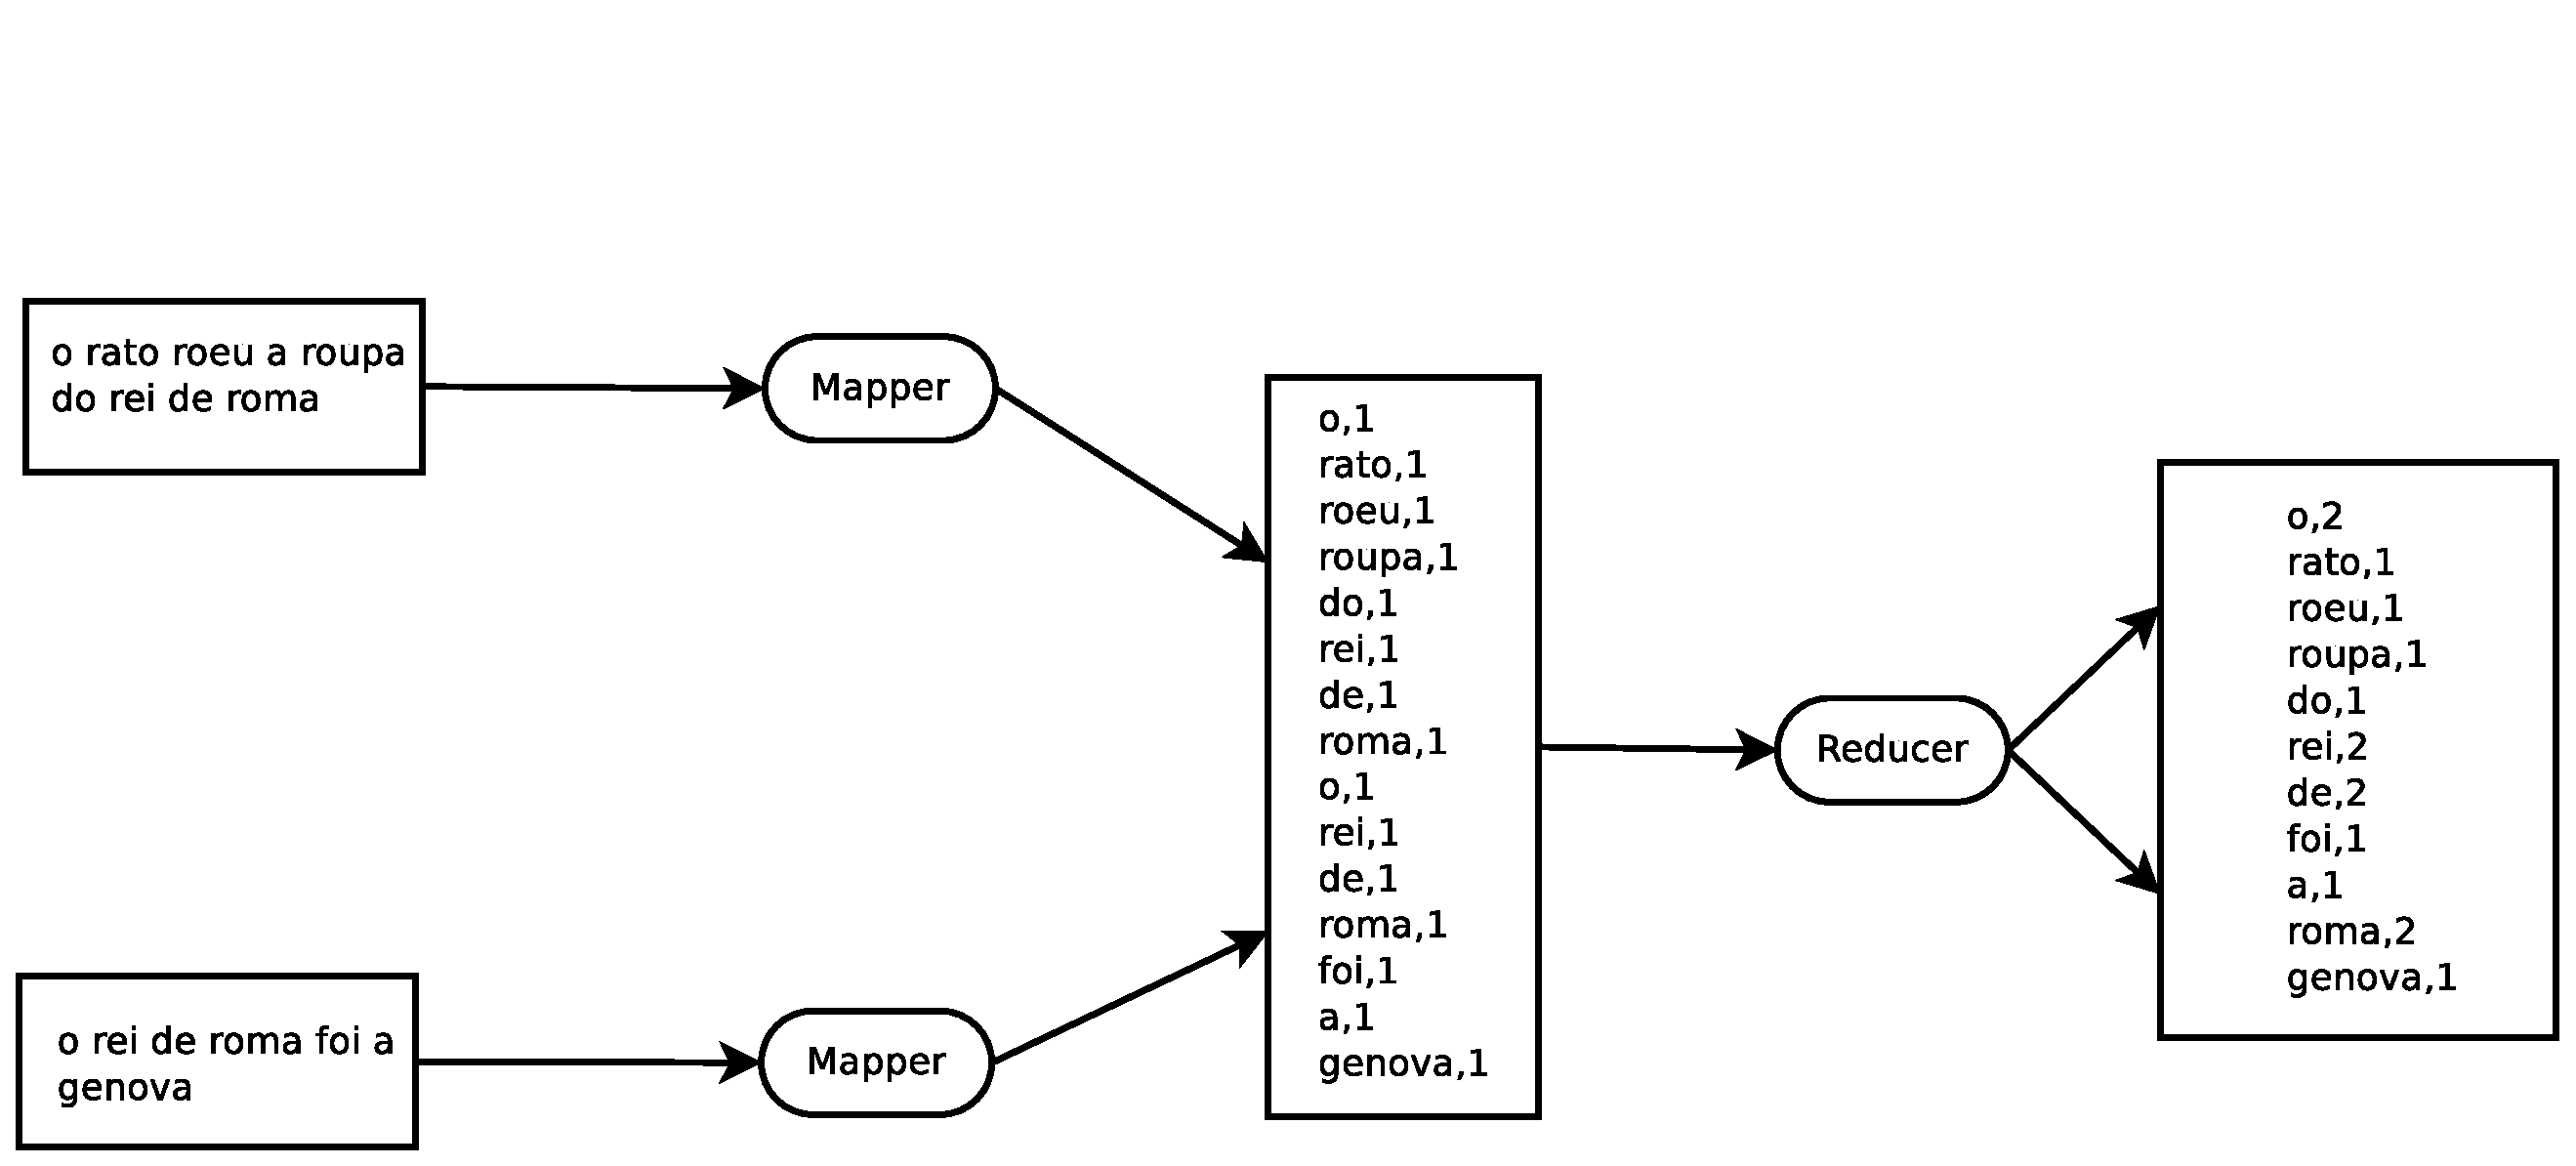
\includegraphics[scale=0.26]{img/exemplo_mapreduce.eps}
				\caption{Problema de contagem de palavras.}
				\label{fig:mapreduce_example}
			\end{figure}
		\end{frame}

\section{Proposta}
	\subsection{Problema}
		\begin{frame}{Problema}
			Solução atual não escalará com:
			\begin{itemize}
				\item Aumento de embarcações;
				\item Aumento da frequência de relatórios de posições (15 minutos / 15 segundos);
				\item Aumento do número de requisições;
				\item Aumento do número de áreas monitoradas.
			\end{itemize}
		\end{frame}

	\subsection{Solução}
		\begin{frame}{Solução - Objetivo}
			Implementar uma solução que seja mais simples de escalar quando a demanda crescer. Tais funcionalidades devem ser escaláveis:
			\begin{itemize}
				\item Busca em área: selecionar posições presentes em uma área;
				\item Busca de interessados: selecionar áreas que contenham uma posição.
			\end{itemize}
		\end{frame}

		\begin{frame}{Solução - Prova de Conceito}
			\begin{itemize}
				\item Busca de interessados;
				\item Assíncrono;
				\item Distribuído;
				\item MapReduce;
				\item Master/Slave;
				\item Scala\footnote{https://scala-lang.org} e Akka\footnote{https://akka.io};
				\item Disponível em https://github.com/chandonbrut/mestrado/gridcomp
			\end{itemize}
		\end{frame}

		\begin{frame}{Solução - Overview}
			\begin{figure}[H]
				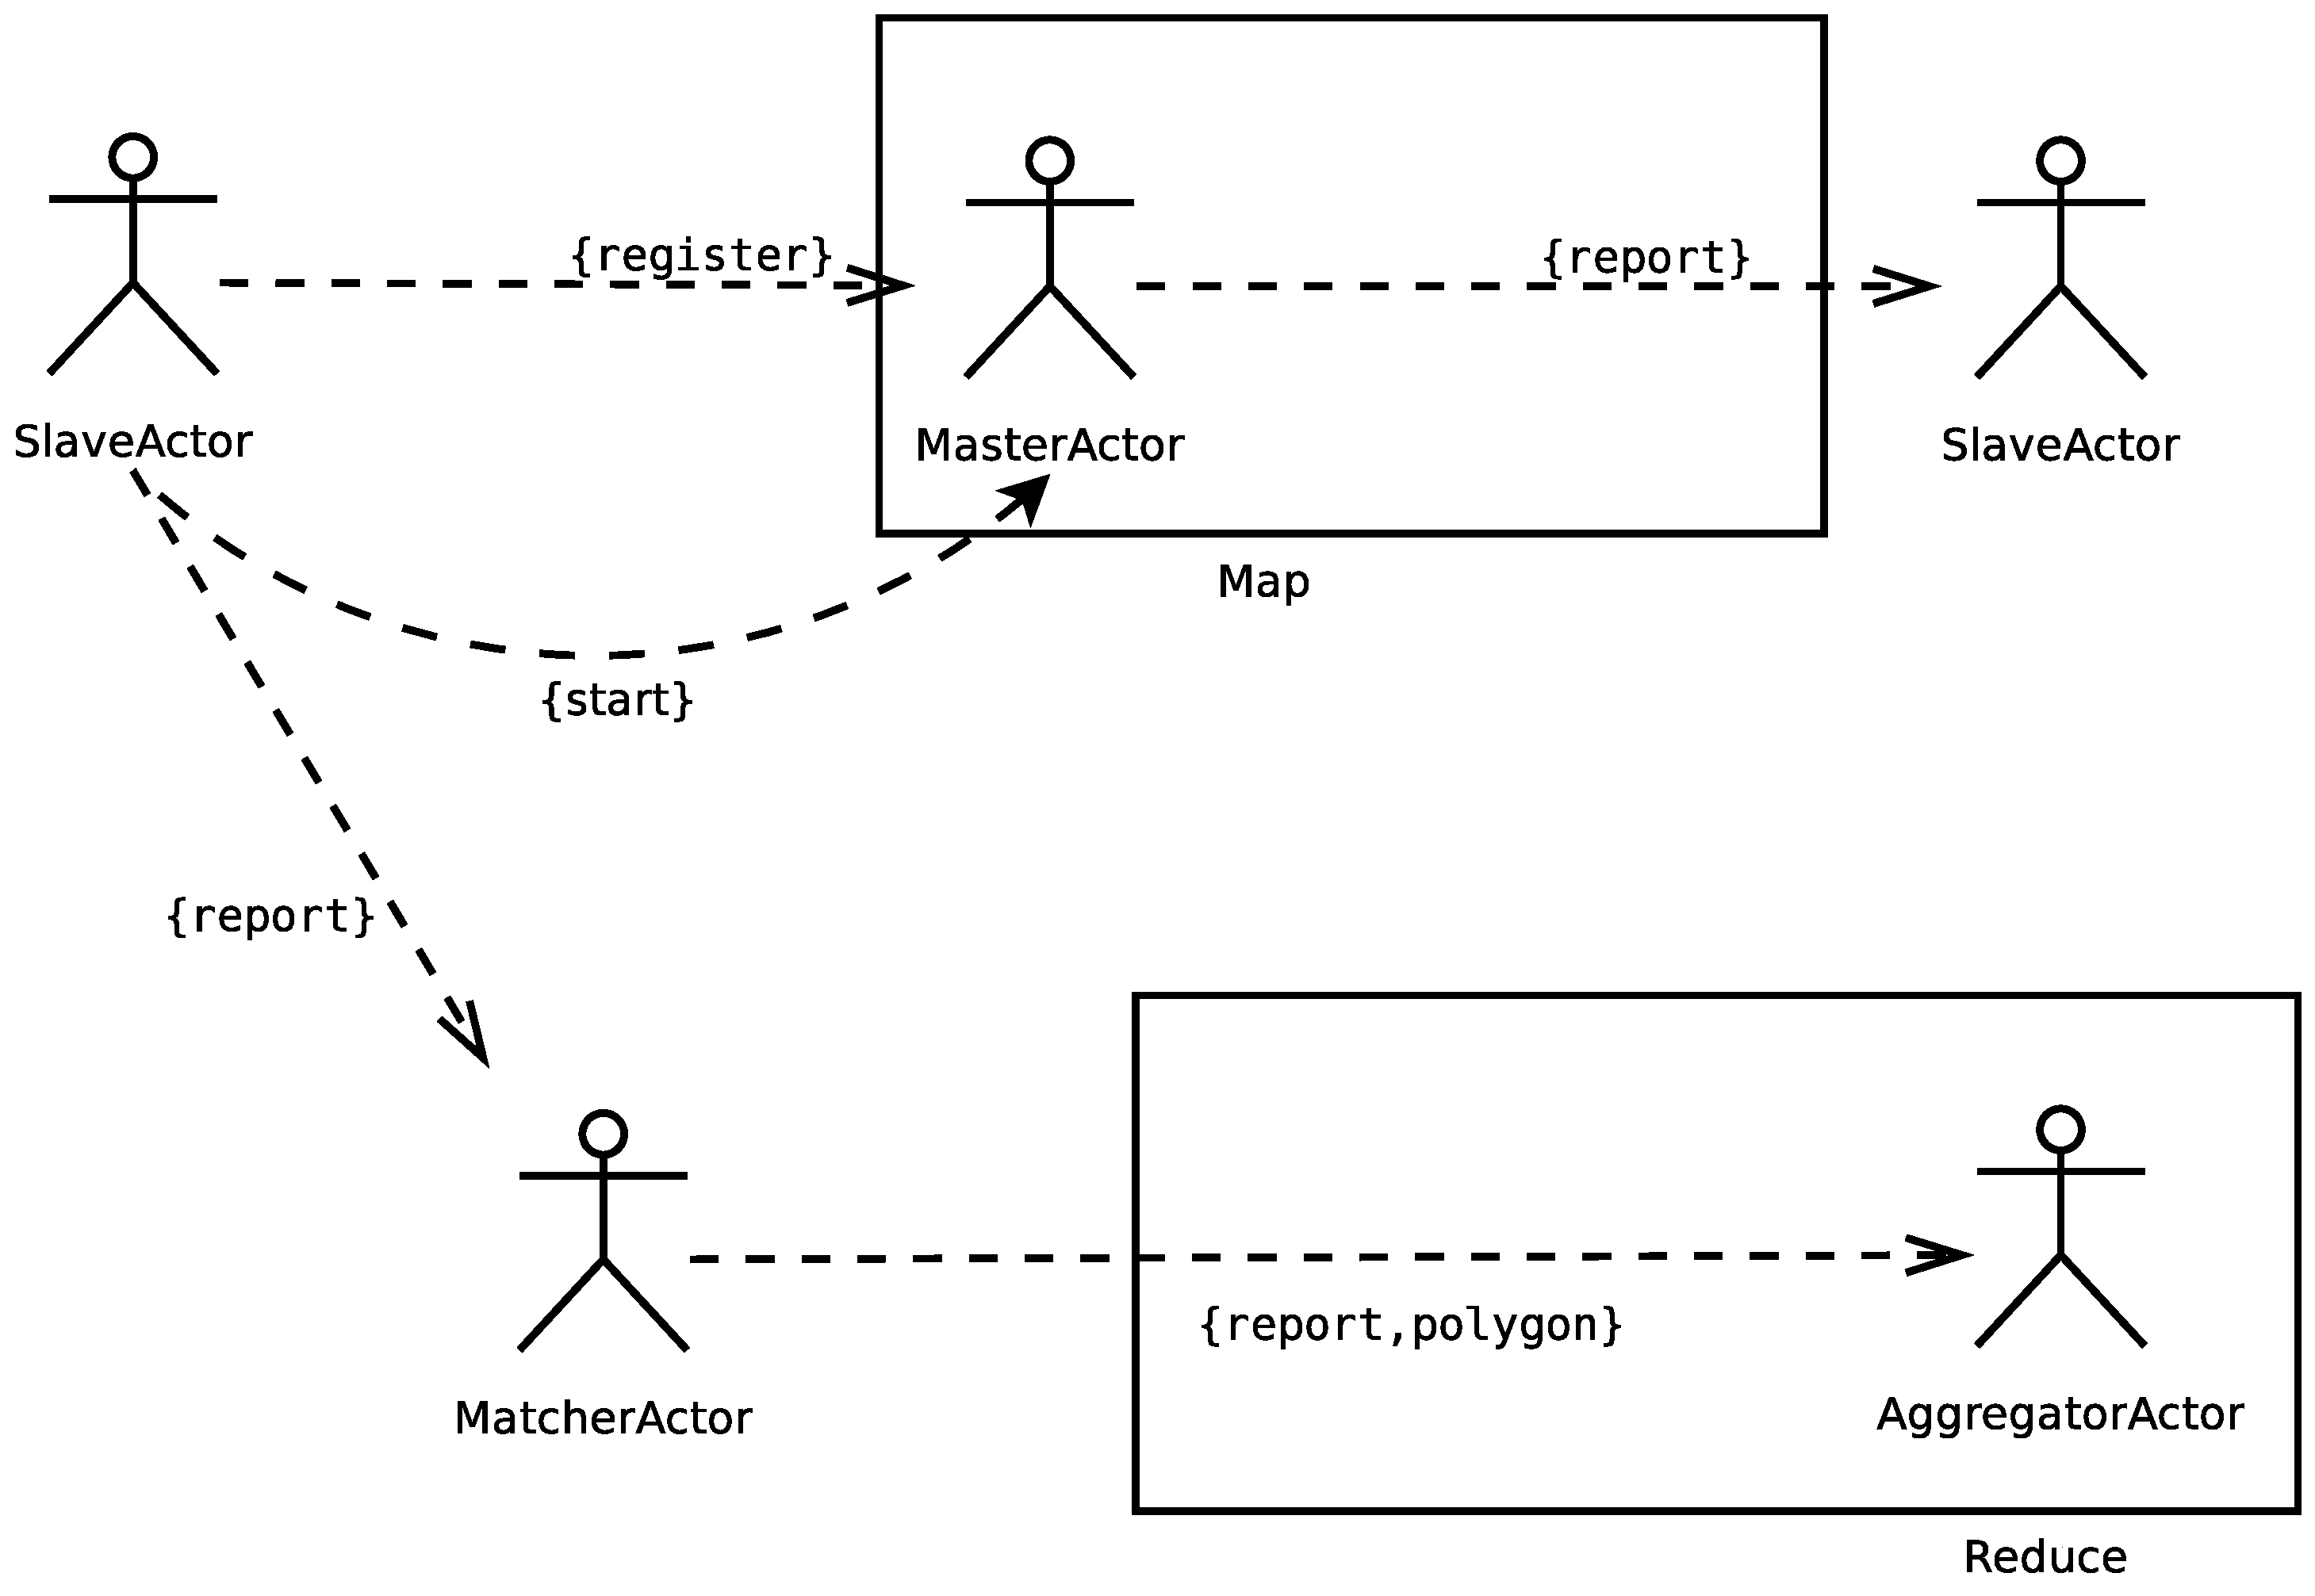
\includegraphics[scale=0.17]{img/actors_overview.eps}
				\caption{Visão geral da solução.}
				\label{fig:actors_overview}
			\end{figure}
		\end{frame}
		
		\begin{frame}{Solução - Overview}
			\begin{figure}[H]
				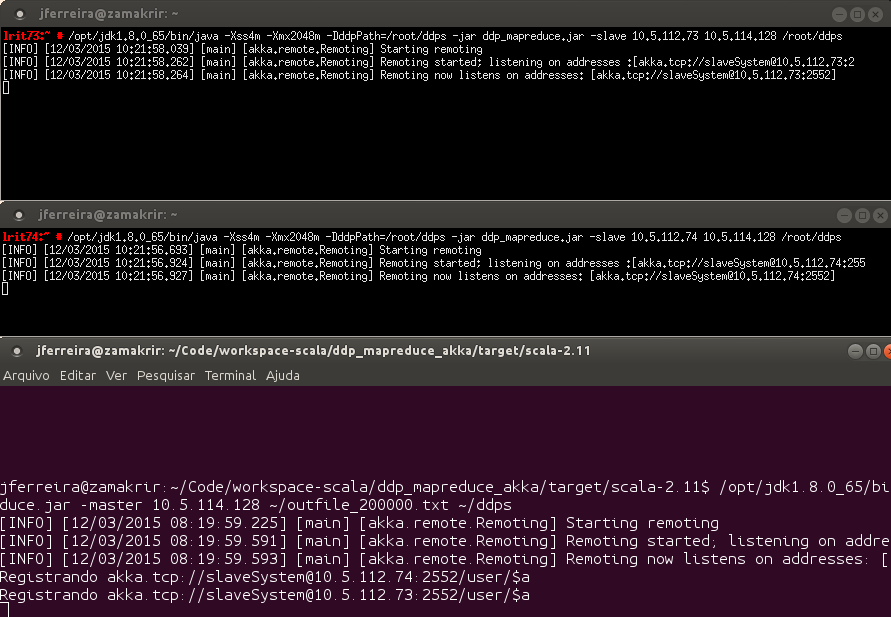
\includegraphics[scale=0.23]{img/screen_mapreduce.png}
				\caption{Exemplo com dois \textit{slaves} conectados.}
				\label{fig:screen_mapreduce}
			\end{figure}
		\end{frame}

\section{Experimento}
	\begin{frame}{Cenário}
		\begin{itemize}
			\item Amostras de posições de navios de tamanhos: 10000, 20000, 100000, 200000;
			\item Cluster com 1, 2 e 3 slaves.
			\item Cada posição deve ser comparada com ~1000 polígonos.
		\end{itemize}
	\end{frame}

	\begin{frame}{Abordagem Sequencial}
		\begin{itemize}
			\item CPU: i7-2600 CPU @ 3.40GHz (8-core)
			\item MEM: java -Xss4m -Xms4096m -Xmx4096m
		\end{itemize}

		\begin{tabular}{| r | c | c |}
		  \hline
		  \#pos & Tempo(s) & Throughput(pos/s) \\
		  \hline			
		 10000 & 231 & 43.29 \\
		 20000 & 460 & 43.48 \\
		 100000 & 2334 & 42.84 \\
		 200000 & 4647 & 43.03 \\
		  \hline  
		\end{tabular}
	\end{frame}

	\begin{frame}{Abordagem Paralela}
		\begin{itemize}
			\item 1 slave; 
			\item CPU: Xeon 5120  @ 1.86GHz (4-core)
			\item MEM: java -Xss4m -Xms2048m -Xmx2048m
		\end{itemize}

		\begin{tabular}{| r | c | c |}
		  \hline
		  \#pos & Tempo(s) & Throughput(pos/s) \\
		  \hline			
		 10000 & 660 & 15.15 \\
		 20000 & 1171 & 17.07 \\
		 100000 & 6062 & 16.49 \\
%		 200000 & 28.0973 & 26.8805 \\
		  \hline  
		\end{tabular}
	\end{frame}

	\begin{frame}{Abordagem Paralela}
		\begin{itemize}
			\item 2 slaves; 
			\item CPU: Xeon 5120  @ 1.86GHz (4-core)
			\item MEM: java -Xss4m -Xms2048m -Xmx2048m
		\end{itemize}

		\begin{tabular}{| r | c | c |}
		  \hline
		  \#pos & Tempo(s) & Throughput(pos/s) \\
		  \hline			
		 10000 & 368 & 27.17 \\
		 20000 & 733 & 26.88 \\
		 100000 & 3507 & 28.51 \\
		 200000 & 6882 & 29.06 \\
		  \hline  
		\end{tabular}
	\end{frame}

	\begin{frame}{Abordagem Paralela}
		\begin{itemize}
			\item 3 slaves; 
			\item CPU: Xeon 5120  @ 1.86GHz (4-core)
			\item MEM: java -Xss4m -Xms2048m -Xmx2048m
		\end{itemize}

		\begin{tabular}{| r | c | c |}
		  \hline
		  \#pos & Tempos(s) & Throughput(pos/s) \\
		  \hline			
		 10000 & 243 & 41.15 \\
		 20000 & 480 & 41.66 \\
		 100000 & 2298 & 43.51 \\
		 200000 & 4659 & 42.92 \\
		  \hline  
		\end{tabular}
	\end{frame}
	
	\begin{frame}{Comparativo}
		\begin{figure}[H]
			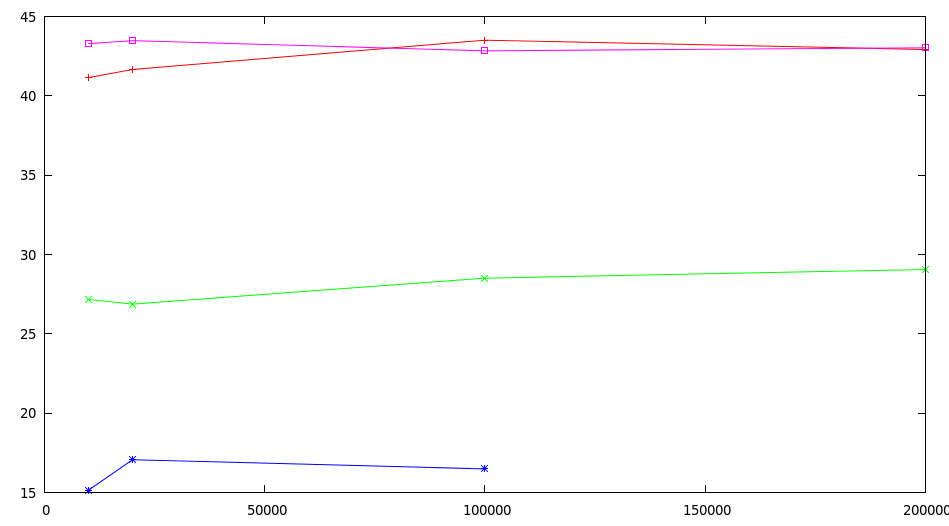
\includegraphics[scale=0.32]{img/graph_throughput.png}
			\label{fig:screen_mapreduce}
		\end{figure}
	\end{frame}

\section{Conclusão}
	\subsection{Resultados}
		\begin{frame}{Resultados}
			\begin{itemize}
				\item Prova de conceito operacional e adequada para trabalhos em lote.
				\item \textit{Slave nodes} podem ingressar e sair a qualquer momento, porém implementação ainda não contempla redistribuição do trabalho.
				\item \textit{Overhead} aceitável considerando a facilidade de escalar recursos.
				\item \textit{Throughput} quase constante em abordagens paralelas.
			\end{itemize}
		\end{frame}

		\begin{frame}{Resultados}
			\begin{itemize}
				\item Apesar do \textit{framework} fornecer os meios para garantir resiliência e recuperação, implementação de fato é complexa.
				\item Facilidades como roteadores de mensagens com diferentes políticas: \textit{RoundRobin}, \textit{SmallestMailbox}, etc.
				\item Desempenho escalando linearmente de acordo com o número de \textit{slaves}.
			\end{itemize}
		\end{frame}

	\subsection{Futuro}
		\begin{frame}{Futuro}
			\begin{itemize}
				\item Implementar um protocolo melhor e tolerância a erros;
				\item Testar com múltiplos \textit{jobs};
				\item Adicionar capacidade de elasticidade com \textit{job} em andamento.
			\end{itemize}
		\end{frame}

\section{Referências}
	\begin{frame}[allowframebreaks]{Bibliografia}
	 	\bibliographystyle{apalike}
		\begin{tiny}
	 		\bibliography{ref} 
	 	\end{tiny}
	\end{frame}

\end{document}